
\begin{figure}[!h]
\centering
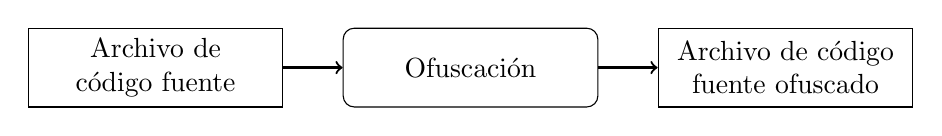
\begin{tikzpicture}[scale=1,
input_output/.style ={rectangle, minimum width=1cm, minimum height=1cm,text centered, text width=3cm, draw=black},
algorithm/.style={rectangle, rounded corners, minimum width=3cm, minimum height=1cm,text centered, text width=3cm, draw=black},
arrow/.style={thick,->,},
]
\node[input_output] (n0) at (1,1) {Archivo de código fuente};
\node[algorithm] (n1) at (5,1) {Ofuscación};
\node[input_output] (n2) at (9,1) {Archivo de código fuente ofuscado};
\draw [arrow] (n0.east) to (n1.west);
\draw [arrow] (n1.east) to (n2.west);
\end{tikzpicture}
\caption{Ofuscación de código fuente}
Fuente: Elaboración propia.
\label{obfuscationSC}
\end{figure}
